% Template for PLoS
% Version 1.0 January 2009
%
% To compile to pdf, run:
% latex plos.template
% bibtex plos.template
% latex plos.template
% latex plos.template
% dvipdf plos.template

\documentclass[10pt]{article}

% amsmath package, useful for mathematical formulas
\usepackage{amsmath}
% amssymb package, useful for mathematical symbols
\usepackage{amssymb}

% graphicx package, useful for including eps and pdf graphics
% include graphics with the command \includegraphics
\usepackage{graphicx}

% cite package, to clean up citations in the main text. Do not remove.
\usepackage{cite}

\usepackage{color} 

% Use doublespacing - comment out for single spacing
%\usepackage{setspace} 
%\doublespacing


% Text layout
\topmargin 0.0cm
\oddsidemargin 0.5cm
\evensidemargin 0.5cm
\textwidth 16cm 
\textheight 21cm

% Bold the 'Figure #' in the caption and separate it with a period
% Captions will be left justified
\usepackage[labelfont=bf,labelsep=period,justification=raggedright]{caption}

% Use the PLoS provided bibtex style
\bibliographystyle{plos2009}

% Remove brackets from numbering in List of References
\makeatletter
\renewcommand{\@biblabel}[1]{\quad#1.}
\makeatother


% Leave date blank
\date{}

\pagestyle{myheadings}
%% ** EDIT HERE **


%% ** EDIT HERE **
%% PLEASE INCLUDE ALL MACROS BELOW

\DeclareMathOperator{\Tr}{tr}
\newcommand{\mcond}{\,\middle\vert\,}
\newcommand{\cond}{\,\vert\,}
\newcommand{\loss}[1]{\mathcal L\left(#1\right)} 
\newcommand{\T}{\intercal}
\newcommand{\E}[2][]{\mathbb E_{#1}\left[ #2\right]}    % expected value
\newcommand{\TODO}[1]{\emph{\small\color{blue}$\langle\langle$#1$\rangle\rangle$}}
\newcommand*\dif{\mathop{}\,d}
\DeclareMathOperator{\rank}{rank}

%% END MACROS SECTION

\begin{document}

% Title must be 150 characters or less
\begin{flushleft}
{\Large
Improved estimates of neural correlations suggest detailed interactions in visual cortex
}
% Insert Author names, affiliations and corresponding author email.
\\
Dimitri Yatsenko$^{1,\ast}$, 
Kre\v{s}imir Josi\'{c}$^{2}$,
Alexander Ecker$^{3,1}$,
Emmanouil Foudarakis$^{1}$,
R.~James Cotton$^{1}$,
Andreas S.~Tolias$^{1}$
\\
\bf{1} Department of Neuroscience, Baylor College of Medicine, Houston, TX, USA
\\
\bf{2} Max Planck Institute of Biological Cybernetics, T\"ubingen, Germany
\\
\bf{3} Department of Mathematics and Department of Biology and Biochemistry, University of Houston, Houston, TX, USA
\\
$\ast$ E-mail: yatsenko@cns.bcm.edu
\end{flushleft}

% Please keep the abstract between 250 and 300 words
\section*{Abstract}
Linear correlations between the spiking activity of pairs of neurons are among the most familiar and useful descriptive statistics of neural activity. Multineuronal recordings provide far richer information than the equivalent number of neuron pairs considered in isolation. For example, the full covariance matrix reveals the partial correlations between pairs of neurons, as well as correlated activity across the entire population. Covariance matrix estimates require large samples for convergence. Convergence  can be improved by regularization, \emph{i.e.}~by imposing some kind of structure.  The optimal regularization must be determined empirically since its performance depends on how the imposed structure captures the underlying interactions. For example, we can use low-rank parameterizations of the covariance matrix to account for correlated input onto many neurons. Conversely, if correlations are a result of a small number of  pairwise linear interactions between the observed neurons, we can sparsify the inverse covariance matrix. We can also use a `sparse+low rank’ inverse covariance representation to account for common fluctuations and pairwise interactions in the recorded population.  

To select the optimal structure of neural correlations in a local neural circuit, we compared the performance of several covariance estimators on the activity of 100--300 neurons in mouse visual cortex: sample covariance, Ledoit-Wolf covariance shrinkage, factor analysis, sparse inverse covariance, and sparse+low-rank inverse covariance. We inferred instantaneous firing rates in 200 ms bins from the somatic calcium signals acquired with fast 3D random-access two-photon microscopy.  Each covariance estimator was optimized and evaluated by cross-validation. As expected, covariance shrinkage reliably outperformed the sample covariance estimate. In turn, factor analysis-based estimates significantly outperformed covariance shrinkage. Yet sparse inverse covariance with or without an additional low-rank component significantly outperformed both factor analysis and shrinkage estimators. The superior performance of the sparse inverse covariance estimator suggests the relative importance of detailed network interactions over common diffuse input in the circuit we studied.


% Please keep the Author Summary between 150 and 200 words
% Use first person. PLoS ONE authors please skip this step. 
% Author Summary not valid for PLoS ONE submissions.   
\section*{Author Summary}
We estimated the covariance matrices of the calcium activity of populations of neurons in the primary visual cortex.  
In the effort to improve the estimate, we imposed several types of sparse structure of the covariance matrix and, using cross-validation, compared the performance for resulting estimators.  

\section*{Introduction}
Pearson correlations between the spiking activity of pairs of neurons, or simply \emph{neural correlations}, are among the most familiar descriptive statistics of neural population activity \cite{Averbeck:2006,Zohary:1994,Kohn:2005,Bair:2001,Renart:2010}.  For example, \emph{noise correlations}, \emph{i.e.}~the correlations of stimulus response variability between pairs of neurons, have been of particular interest.  Noise correlations can have profound theoretical implications for stimulus coding \cite{Zohary:1994,Abbott:1999,Averbeck:2006,Berens:2011,Ecker:2011}, and have been interpreted to indicate detailed and specific functional organization. Such interpretation is supported by a series of discoveries of nontrivial relationships between neural correlations and other aspects of circuit organization such as the physical distance separating the neurons \cite{Smith:2008,Denman:2013}, their synaptic connectivity and stimulus tuning similarity \cite{Kohn:2005,Ko:2011}, cortical layer specificity \cite{Hansen:2012,Smith:2013}, cell-type specificity (?), progressive changes in development and in learning \cite{Golshani:2009}, changes due to sensory stimulation and global brain states \cite{Goard:2009,Kohn:2009,Ecker:2010,Renart:2010}, and others.

However, neural correlations do not come with ready or unambiguous mechanistic interpretations.  Theoretical and simulation studies have shown that neural correlations may arise at various temporal scales from combinations of multiple underlying mechanisms.  These include direct synaptic interactions, common or correlated inputs, shared sensory noise, chains of multiple synaptic connections, oscillations, top-down modulation, and background network activity \cite{Perkel:1967b,Shadlen:1998,Salinas:2001,Ostojic:2009,Rosenbaum:2011}.

Early studies of neural correlations were based on measurements from isolated pairs of neurons and their impact on coding was extrapolated to entire populations \cite{Shadlen:1998,Zohary:1994}.  Multineuronal recordings allow estimation of covariance matrices of large populations of neurons.  Such estimates provide more information than the equivalent number of pairwise correlations assessed in isolation. Indeed, the correlation matrix is greater than the sum of its parts: it can be transformed into other representations that accentuate different aspects of the correlation structure and may suggest different mechanistic interpretations. For example, the eigenvalue decomposition of the covariance matrix expresses shared correlated activity components across the population; common fluctuations of population activity may be accurately represented by just a few principal components but will affect all correlation coefficients. In contrast, the off-diagonal elements of the inverse of the correlation matrix constitute scaled partial correlations between neuron pairs, which reflect their specific linear dependencies, after accounting for the activity of all the other recorded cells; a strong interaction between a pair of neurons may be expressed by a single partial correlation but its effects may propagate to multiple correlations and eigenvalues.   The inverse of the covariance matrix plays an important role in decoding schemes such as linear discriminant analysis, for example.  The mutliple  representations of the covariance matrix with their alternative interpretations add both complications and opportunities into the search for fundamental regularities in neural population activity. 

With large numbers of recorded cells, the usual estimations of the covariance matrix from finite recordings become ill-conditioned. Numerical instabilities arise because, as the amount of recorded data increases only linearly, the number of free coefficients to be estimated in any parameterization of the covariance matrix increases quadratically. 
For example, the large eigenvalues of large sample covariance matrices are biased upward while small eigenvalues are biased downward \cite{Ledoit:2004}. Similarly, the coefficients of the inverse covariance matrix require larger sample sizes to be estimated accurately from high-dimensional data than low-dimensional data.

With this study, we pursue two related goals: 
\begin{enumerate}
	\item Devise more efficient estimators of neural covariance matrices in recordings from large populations of neurons.
	\item Aid interpretation of neural covariance matrices.
\end{enumerate}

To select the best covariance matrix estimate for a specific neural circuit, we evaluate the performance of four estimators using different regularization schemes, each motivated by  a different hypothesis for the origin of neural correlations. \emph{Regularization} is the deliberate biasing the solution toward a simplified, low-dimensional (`sparse') \emph{target estimate} \cite{Schafer:2005,Bickel:2006}.
Regularized estimators allow reaching a favorable tradeoff between bias and variance in order to minimize the total error.
Strikingly, some improvement can be produced even when the target estimate is chosen arbitrarily, which is sometimes described as ``Stein's phenomenon'' after its discoverer \cite{Stein:1956}.   However, when a sparse target estimate does happen to match the dominant features of the true covariance matrix, it will induce relatively little bias while retaining low variance.  For example, some covariance estimators have been motivated by a specific model of the underlying process such as single-factor models of the stock market, for example \cite{Ledoit:2003}. 
Since the true covariance structure is not known in practice, the performance of estimators is evaluated by how well their performance generalized to new data, outside the training sample by cross validation, for example. 


We compared the performance of several covariance estimators for spatially compact groups of 150--300 neurons in layers 2--4 in mouse primary visual cortex during visual stimulation.   The performance of the estimators was evaluated by computing the mean squared error between the optimized covariance estimate fitted to training data and the non-regularized covariance matrix from a separate test data set.  Low-rank covariance estimates performed significantly better than shrinkage estimators, but estimators with sparse partial correlations were more efficient still. Typically, between 3 and 16\% of neuronal pairs were connected by non-zero partial interactions.  Mixed sparse estimators with sparse partial correlations and low-rank components performed comparably. 



% Results and Discussion can be combined.
\section*{Results}
\subsection{Data acquisition}
Describe the two-photon experiment, refer to Fig.\;1

\subsection*{Basic concepts}
Let $x(t) \in \mathcal X, t=1\ldots,n$ denote a sample of consecutive observations of population activity of $p$ neurons in time bins $t$.  
The activity of each neuron is denoted by the real-valued firing rate, thus  $\mathcal X = \mathbb R^{p\times 1}$.  
For example, in our applicaiton, the firing rate is estimated from somatic calcium fluorescence signals with the mean stimulus response subtracted, making it possible for elements of $x(t)$ to take on negative and non-integer values. 

We do not assume that the observations $x(t)$ are independently distributed. Rather, the data generating process is assumed to be \emph{ergodic}, \emph{i.e.}\;described by a \emph{true distirbution} $F: \mathcal X \mapsto  \mathbb [0, 1]$ (cumulative) over long periods of time such that the \emph{empirical distribution} $\hat F_n$ from a given sample will convege to $F$ with increasing sample size $n$.

Formally, the emprical distribution is defined as \TODO{this may be unecessary, but I leave it for now.}
\begin{equation}
\hat F_n(x) = \frac 1 n \sum\limits_{t=1}^n \mathbf{1}(x \ge x(t))
\end{equation}
where $\mathbf 1(x \ge x(t))$ is the indicator function which equals 1 when all elements of $x$ are greater than the corresponding elements of $x(t)$ and 0 otherwise. \TODO{KJ: Are you using cumulative distributions to avoid binning? DY: Yes. Many theorems such as Glivenko-Catelli Theorem and Skorohod's Representation are proven using  cumulative representation. The empirical distribution is nearly always represented in its cumulative form. Expressing convergence is requires binning or using cumulative; the latter is simpler.}

And, for an ergodic process, $\max\limits_{x\in\mathcal X} \left|\hat F_n(x) - F(x)\right| \to 0$ as $n$ increases.

The true covariance matrix $\Sigma \in \Theta$ is defined as a function of $F$:
\begin{equation}
\Sigma = \int\limits_{z\in\mathcal X} (z - \mu)(z - \mu)^\T \dif F(z)
\quad\mbox{where}\;
\mu = \int\limits_{z\in\mathcal X} z \dif F(z)
\end{equation}
The domain $\Theta$ is the set of all positive-definite $p\times p$ matrices, which is a cone in $\mathbb R^{p\times(p+1)/2}$.

But the usual estimator of the true covariance matrix $\Sigma$ is  the sample covariance matrix:
\begin{equation}
\hat\Sigma_0 =  \frac 1 {n-c} \sum\limits_{t=1}^n (x(t) -\hat\mu) (x(t) - \hat\mu)^\T
\quad\mbox{where}\;
\hat\mu = \frac 1 n \sum\limits_{t=1}^n x(t)
\end{equation}
where $c$ is the sum of temporal correlations \TODO{there must be a better description of this}. For independent observations, $c=1$;  $c>1$ when nearby samples are correlated; the value of $c$ can be estimated from the data.
\TODO{Under the Gaussian loss, $\mathcal L_g$ (\ref{eq:GaussLoss}) the scaling is irrelevant, so we will not spend any time talking about the scaling.  But it would be important if we used $\mathcal L_e$ (\ref{eq:MSE}).} 

$\hat\Sigma_0$ is designed to be unbiased such that $\mathbb E\left[\hat\Sigma_0\right]=\Sigma$.
Here and througout, $\mathbb E[\cdot]$ denotes the expected value under the  unknown true distribution $F$. All variables with a hat (\emph{e.g.}\;$\hat \Sigma_0,\hat \mu$) are functions of the empirical distribution $\hat F_n$, which itself is a random variable.

%Nonlinear functions of an unbiased estimate can be biased: $\mathbb E\left[\hat\Sigma_0\right]=\Sigma \centernot\implies  E\left[\varphi(\hat\Sigma_0)\right]=\varphi(\Sigma)$.  For example, if $u_{\max}(S)$ is the largest eigevalue of square matrix $S$, then $\mathbb E\left[u_{\max}(\hat\Sigma_0)\right] > u_{\max}(\Sigma)$. Some covariance matrix estimators are designed to correct for the eigenspectrum bias at the cost  of adding bias to covariance coefficients \cite{Ledoit:2004}.




\subsection*{Loss and risk}
The optimization of a covariance matrix estimate $\hat\Sigma$ is performed with respect to a \emph{loss function} $\mathcal L(\hat\Sigma,\Sigma)$, which expresses the discrepancy between $\hat\Sigma$ and $\Sigma$ and attains its minimum when $\hat\Sigma=\Sigma$.  
Then \emph{excess loss}  
\begin{equation}
\ell(\hat\Sigma,\Sigma) = \mathcal L(\hat\Sigma,\Sigma)-\mathcal L(\Sigma,\Sigma)
\end{equation}
assumes zero at its minimum.

A particularly useful loss function is the mean squared error (MSE), which is proportional to the square of the Frobenius  norm $\|\cdot\|_F$ of the difference between the two matrices: 
\begin{equation}\label{eq:MSE}
\mathcal L_e(\hat\Sigma,\Sigma) =\frac 1 p \|\hat\Sigma-\Sigma\|_F^2 = \frac 1 p \Tr\left((\hat \Sigma-\Sigma)(\hat\Sigma-\Sigma)^\T\right)
\end{equation}
Since $\mathcal L_e(\Sigma,\Sigma) \equiv 0$, the MSE is its own excess loss: $\ell_e(\hat\Sigma,\Sigma) \equiv \mathcal L_e(\hat\Sigma,\Sigma)$.

The Gaussian loss function $\mathcal L_g$  arises from the theory of multivariate normal distributions. When observations are identically and independently distributed according to a multivariate normal distribution with zero means, the log likelihood of the covariance matrix $\Sigma$ with $\hat\Sigma = \frac 1 n \sum\limits_{t=1}^n x(t) x(t)^\T$ is  
\begin{equation}
L\left(\Sigma \mid \hat\Sigma\right) = -\frac n 2 \ln(2\pi) - \frac n 2 \ln \det \Sigma - \frac n 2 \Tr(\Sigma^{-1} \hat \Sigma)
\end{equation}
Then $\mathcal L_g$ is constructed by rescaling $L\left(\Sigma \mid \hat\Sigma\right)$ and dropping the constant term:
\begin{equation}\label{eq:GaussLoss}
\mathcal L_g(\hat\Sigma,\Sigma) 
=  -\frac 2 {pn} L\left(\Sigma \mid \hat\Sigma \right) - \frac 1 p \ln(2\pi) 
\equiv  \frac 1 p\left(\ln \det \hat \Sigma + \Tr(\hat \Sigma^{-1}) \right) 
\end{equation}
The corresponding excess loss 
\begin{equation}
\ell_g(\hat\Sigma,\Sigma) = \mathcal L_g(\hat\Sigma,\Sigma) - \mathcal L_g(\Sigma,\Sigma)  
= \frac 1 p \left(-\ln \det (\hat \Sigma^{-1} \Sigma) + \Tr(\hat \Sigma^{-1}\Sigma)\right) - 1
\end{equation}
is known as \emph{entropy loss} \cite{James:1961}. \TODO{The order of the operands is reversed. Check that it's okay.}

Despite the fact that entropy loss is derived from normal theory, the choice of a loss function is not equivalent to assuming a specific form of $F$. The loss function measures the discrepancy between distribution parameters rather than the distance between the distributions themselves. \TODO{explain Bregman divergence?} 

The expected value of excess loss is the \emph{estimator risk}:
\begin{equation}\label{eq:risk}
r = \mathbb E\left[\ell(\hat\Sigma,\Sigma)\right]
\end{equation}
The estimator risk is the primary quality criterion for covariance estimation. Estimator $\hat\Sigma_a$ is considered more \emph{efficient} than estimator $\hat\Sigma_b$ if $\hat\Sigma_a$ has lower risk for the given sample than $\hat\Sigma_b$.   \TODO{explain that the risk depends not only on $\hat\Sigma$ but also on the distribution of $\Sigma$ in the specific domain.}

\subsection*{Cross validation}
In practice, the true covariance matrix $\Sigma$ is not accessible and the estimator risk $r$ must be estimated from data. This requires a separate \emph{validation} empirical distribution $\hat F_m^\prime$ of $m$ observations sampled from $F$ independently of the \emph{training} distribution $\hat F_n$. 
Then let  $\hat \Sigma_0^\prime$ be the sample covariance obtained from $\hat F_m^\prime$. 

Then the \emph{empirical loss} of $\hat\Sigma$ is $\mathcal L(\hat\Sigma,\hat\Sigma_0)$ and its expectation is the \emph{empirical risk}  
\begin{equation}
\hat r = \mathbb E\left[\mathcal L(\hat\Sigma,\hat\Sigma_0^\prime)\right]
\end{equation}

 The two loss functions $\mathcal L_e(\hat\Sigma,\Sigma)$ and $\mathcal L_g(\hat\Sigma,\Sigma)$ are particularly suitable for risk estimation thanks to their linearity with respect to $\Sigma$ in the sense that 
\begin{equation}
\mathcal L\left(\hat\Sigma,\alpha S_1 + (1-\alpha)S_2\right) 
\equiv 
\alpha\mathcal L(\hat \Sigma,S_1) + (1-\alpha)\mathcal L(\hat \Sigma,S_2)
\end{equation}
which allows bringing the expectation inside the empirical loss function:
\begin{equation}
\hat r = 
\mathbb E\left[ \mathcal L(\hat\Sigma, \hat\Sigma_0^\prime) \right] 
=
\mathbb E\left[ \mathcal L\left(\hat\Sigma, \mathbb E\left[\hat\Sigma_0^\prime\right]\right) \right] 
=
\mathbb E\left[ \mathcal L(\hat\Sigma, \Sigma) \right] 
= 
r + \mathcal L(\Sigma,\Sigma)
\end{equation}
This means, that the empirical loss $\mathcal L(\hat\Sigma,\hat\Sigma_0^\prime)$ is an unbiased estimate of the estimator risk $r$ (up to a constant offset): minimization of the empirical loss implies minimization of the true estimator risk. 

Recording a separate independent validation sample is usually not sensible.  Instead, the recorded data are split into a training sample and validation sample. In $K$-fold \emph{cross-validation} the data are split into $K$ roughly equal-sized subsets. Each subset then successively serve as the testing sample while the remainder of the data serves as the training sample.  This procedure produces $K$ estimates of the  risk, which are then averaged together to produce a better averaged estimate.


\subsection*{Bias/variance decomposition}
The estimator risk (\ref{eq:risk}) can be decomposed into \emph{approximation error} or \emph{bias}   
\begin{equation}
b^2 = \ell \left( \mathbb E[\hat \Sigma],\Sigma\right)
\end{equation}
and \emph{estimation error} or \emph{variance}
\begin{equation}
\varepsilon^2 = \mathbb E \left[ \ell\left(\hat \Sigma, 
\mathbb E[\hat \Sigma]\right) \right]
\end{equation}

Under the MSE loss function $\mathcal L_e$ (\ref{eq:MSE}), the decomposition is the simple sum $r = b^2 + \varepsilon^2$. 
Under other loss functions, $r$ is an increasing function of both $b^2$ and $\varepsilon^2$ although not generally a simple sum.  
\TODO{As far as I know, the terms `bias' and `variance' are only applicable under a quadratic loss function  like $\mathcal L_e$.  Under other loss functions, we may need to use approximation/estimation error.} 

The sample covariance matrix $\hat\Sigma_0$ has zero bias but high variance. Other estimators may be biased but have lower estimation error and potentially lower risk.


\subsection*{Regularization}

\emph{Regularization} is the deliberate biasing (`shrinkage') of the unbiased estimate toward a less variable low-dimensional \emph{target estimate} $\hat T$ in order to minimize the estimator risk by striking a favorable balance between bias and variance.
A regularized covariance matrix estimator must solve two problems: (a) choose and fit the target covariate estimate $\hat T$ and (b) mix $\hat\Sigma_0$ with $\hat T$ by the optimal amount. 
Regularized covariance matrix estimates can be generally expressed as 
\begin{equation}
\hat\Sigma_{d,\lambda} = mix(\Sigma_0,\hat T_{\hat d},\hat\lambda) 
\end{equation}
where $\hat d$ indicates the choice of the target estimate from the family of target estimates $\hat T_d$. $mix(\cdot,\cdot,\hat\lambda)$ is the mixing function of $\hat\Sigma_0$ and $\hat T_{\hat d}$ in proportion controlled by $\hat \lambda$. Both $\hat d$ and $\hat \lambda$ must be calculated from the training sample. 

A number of regularization schemes have been developed, which differ by their target estimates and mixing functions.    Curiously, \emph{some} improvement can be produced with an arbitrary target estimate as long as its variance is lower than that of $\hat\Sigma_0$.  The perplexing phenomenon that estimates can be improved by a bias toward an arbitrary less variable target is known as \emph{Stein's paradox} \cite{Efron:1977}.   \TODO{This point can be untuitive.  For example, \cite{Varoquaux:2012} misrepresents the effect of regularization by stating that regularization removes the upward bias of correlations in the sample covariance matrix. In reality, regularization should start with an unbiased estimator and bias it toward a low-variance target so that the estimation risk is reduced.} However, if a family of target estimates can capture the underlying regularities in the covariance structure of a specific system with a small number of parameters, biasing the estimate toward these targets ought to produce a greater reduction in estimator risk. 

In this study, we evaluate four regularized estimators whose target estimates correspond to the graphical models in Figure \ref{fig:02}: diagonal (A), multifactor (B), sparse partial correlations (C), and sparse  partial correlations with latent units (D).  The following describe each regularization scheme separately.

\begin{figure}[htp]
\centering
\includegraphics[width=0.5\textwidth]{figures/Figure2.pdf}
\caption{
Graphical models corresponding to the low-dimensional targets of the four regularization schemes used in the paper.
\textbf{A}: A diagonal matrix corresponds to a Gaussian graphical model with no dependencies. 
\textbf{B}: In factor analysis, observed nodes are assumed to be influenced by several latent units (``factors") but are otherwise independent. 
\textbf{C}: In the Gaussian graphical model (also known as the Gaussian Markov Field), correlations arise from sparse pairwise linear interactions between visible units. 
\textbf{D}: In the Gaussian graphical model with latent units, correlations arise  between pairs of nodes 
}\label{fig:02}
\end{figure}


\subsection*{Regularization}
Under many loss functions\footnote{
The strict equality in Eq.~\ref{eq:bias-variance} does not hold under the loss function in Eq.~\ref{eq:loss}. 
However, the equality does hold for its close cousin, Stein's \emph{entropy loss}, which only differs by the order of its arguments and a constant offset: $\mathcal L_s(\hat\Sigma,\Sigma) \equiv \loss{\Sigma,\hat\Sigma} - \loss{\Sigma,\Sigma}$. 
This defficiency presents no difficulty because we minimize the risk directly, without assessing the two error components individually. 
The bias-variance decomposition is presented here to motivate the use of regularization.}, 
the estimator's risk can be decomposed as the sum
\begin{equation}\label{eq:bias-variance}
    r = b + \varepsilon
\end{equation}
of \emph{approximation error} (``bias'' or systematic error)
\begin{equation}
   b = \loss{\bar\Sigma,\Sigma}
\end{equation}
and \emph{estimation error} (``variance'') 
\begin{equation}
   \varepsilon = \E[\hat\Sigma]{\loss{\hat\Sigma, \bar\Sigma}}
\end{equation}
where $\bar\Sigma = \E{\hat\Sigma}$ is the expected value of the estimate. 

The unbiased estimator $\hat\Sigma_0$ makes $\bar\Sigma=\Sigma$ and thereby minimizes the approximation error, but may be excessively susceptible to sample noise and result in high estimation error.

The estimator risk can be reduced by \emph{regularization}. Regularization is the deliberate biasing (\emph{``shrinkage''}) of the estimate toward a low-dimensional, less variable \emph{target estimate} \cite{Bickel:2006,Ledoit:2004}. 
A regularized estimator solves the bias-variance tradeoff to produce a biased but less variable estimates aiming to minimize the estimator's risk.  
Various regularization schemes focus on the dimensionality reduction part \TODO{rephrase} by selecting the optimal target estimate from a family of estimates with reduced dimensionality \cite{findit}.  
Other estimators only shrink the sample covariance matrix toward a single target estimator \cite{Schafer:2005}. 
Yet other regularizers effectively combine shrinkage and dimensionality reduction \cite{findit}.

\subsection*{Estimator A: Shrinkage toward diagonal}
The most popular covariance regularization schemes use diagonal target estimates and linear shrinkage toward the target.  For example, the target could be the identity matrix:  
\begin{equation}
\hat T = \hat v I
\end{equation}
where $\hat v = \frac 1 p \sum\limits_{i=1}^p(\hat\Sigma_0)_{ii}$ is the mean sample variance. 

Alternatively, the target could contain the sample variances:
\begin{equation}
\hat T= \hat\Sigma_0 \circ I 
\end{equation}
where $\circ$ is the entrywise matrix product.

Finally, the target could be a linear mixture of the common variance and independent variance targets
\begin{equation}
\hat T_{\hat\eta} = (1-\hat\eta)(\hat\Sigma_0 \circ I) + \hat\eta\hat v I
\end{equation}

The regularized estimator is the linear mixture of $\hat\Sigma_0$ and $\hat T_{\hat\eta}$:
\begin{equation}
\hat\Sigma_{\hat\eta,\hat\lambda} = (1-\hat\lambda)\hat\Sigma_0 + \hat\lambda \hat T_{\hat\eta} 
\end{equation}

The hyperparameters $\hat\eta$ and $\hat\lambda$ must be estimated from the data.  Under the MSE loss function $\mathcal L_e$ (\ref{eq:MSE}), the optimal values of $\hat\eta$ and $\hat\lambda$ can be estimated analytically \cite{Ledoit:2004,Schafer:2005,Schaefer:2010}. However, these estimates are no longer optimal under the Gaussian loss $\mathcal L_g$. \TODO{I have tested this and there was a substantial difference in both synthetic and empirical data}  When an analytical solution for optimal hyperparameters is not available, the optimal values can be found by cross validation, entirely within the the training sample. \TODO{explain nested cross-validation in more detail?} \TODO{KJ: Yes - see above.}

\TODO{KJ: I am confused.  This suggests that you are getting different results using the two different loss functions.
However, there was no argument yet that either gives us more relevant information about the underlying distribution
if we do not assume Gaussianity, for instance.  I would argue that the Gaussian loss is better, but this is simply 
because the Euclidean metric is not appropriate on the cone of positive semidefinite variances.  As the 
discussion we have been having with Alex demonstrates, this is a point that needs to be explained clearly.}

\TODO{Describe how the empirical loss is convex in the hyperparameters in this case}

\subsection*{Estimator B: Shrinkage toward a factor model}
For estimator B, the target is a factor model, composed as the sum of a low-rank component $\hat L_{\hat d}\hat L_{\hat d}^\T$ and a diagonal matrix $\hat \Psi$:
\begin{equation}
\hat T_{\hat d} = \hat L_{\hat d} \hat L_{\hat d}^\T + \hat\Psi
\end{equation}
Here $\hat L_{\hat d}$ is an $p\times\hat d$ matrix and $\hat\Psi$ is diagonal.  

If $F$ were assume to be multivariate normal \TODO{or other distributions that are defined by linear dependencies}, the factor model is corresponds to the graphical model (\ref{fig:02}B) where the activity of all neurons are dependent only $\hat d$ latent units. This suggest a mechanistic interpretation in which the interactions between neurons are insignificant compared to the influence of inputs outside the recorded circuit.

Just as with Estimator A, Estimator B is allowed to commit to the low-dimensional target only partially: the overall estimate is the linear mixture of the sample covariance and the target
\begin{equation}
\hat\Sigma_{\hat d,\hat\lambda} = (1-\hat\lambda)\hat\Sigma_0 + \hat  T_{\hat d}
\end{equation}

\TODO{Check \cite{Ledoit:2003,Fan:2011,Fan:2006}}

\subsection*{Estimator C: Sparse inverse}
Assuming that $x$ is distributed normally, the inverse of the covariance matrix or \emph{precision matrix} $K=\Sigma^{-1}$ has special significance: zeros in the precision matrix indicate conditional independence between the corresponding pairs. To see this, let $x=(x_1,\ldots,x_p)^\T \sim g\left(x\cond K\right)$
\begin{equation}
g\left(x\cond K\right) = \frac 1 {Z(K)} \exp\left(-\frac 1 2 \sum\limits_{i=1}^p\sum\limits_{j=1}^p  K_{ij} x_i x_j\right)
\end{equation} 
If $K_{12}\equiv K_{21} = 0$, then the joint distribution of $x_1$ and $x_2$, conditioned on $x_3=a_3,\ldots,x_p=a_p$ can be decomposed as product of independent distributions of $x_1$ and $x_2$: 
\begin{equation}
\begin{split}
g\left( x_1, x_2 \cond K, x_3=a_3,\ldots,x_p=a_p\right) &=
\frac 1 {Z(K)} \exp\left(-\frac 1 2 \sum\limits_{i=3}^p\sum\limits_{j=3}^p  K_{ij} a_i a_j \right)\times
\\
 &  \exp\left( -\frac 1 2\left( K_{11} x_1^2 +  x_1\sum\limits_{i=3}^p K_{1i}a_i \right)  \right)
\\
 &  \exp\left( -\frac 1 2\left( K_{22} x_2^2 +  x_2\sum\limits_{i=3}^p K_{2i}a_i \right)  \right)
\end{split}
\end{equation}


\cite{Dempster:1972,Meinshausen:2006,Friedman:2008}

\subsection*{Estimator D: Sparse inverse with latent units}
\cite{Ma:2013} 


\subsection{Simulation}
To illustrate,

\textbf{Figure 2.}{
Simulation results. 
\textbf{A}: A $100 \times 100$ covariance matrix without a low-dimensional structure, a sample covariance with n=2000, distributions of true and sample correlation coefficients, eigenspectra of true and sample covariances.
\textbf{B}: A similar covariance matrix with 8 factors.
\textbf{C}: A similar covariance matrix with sparse inverse. 
\textbf{D}: A similar covariance matrix with sparse + low-rank inverse with 3 latent units.
\textbf{E}: Risk convergence rates
}\label{fig:02}

\subsection*{In visual cortex, Estimator D dominates}
\begin{figure}[htp]
\centering
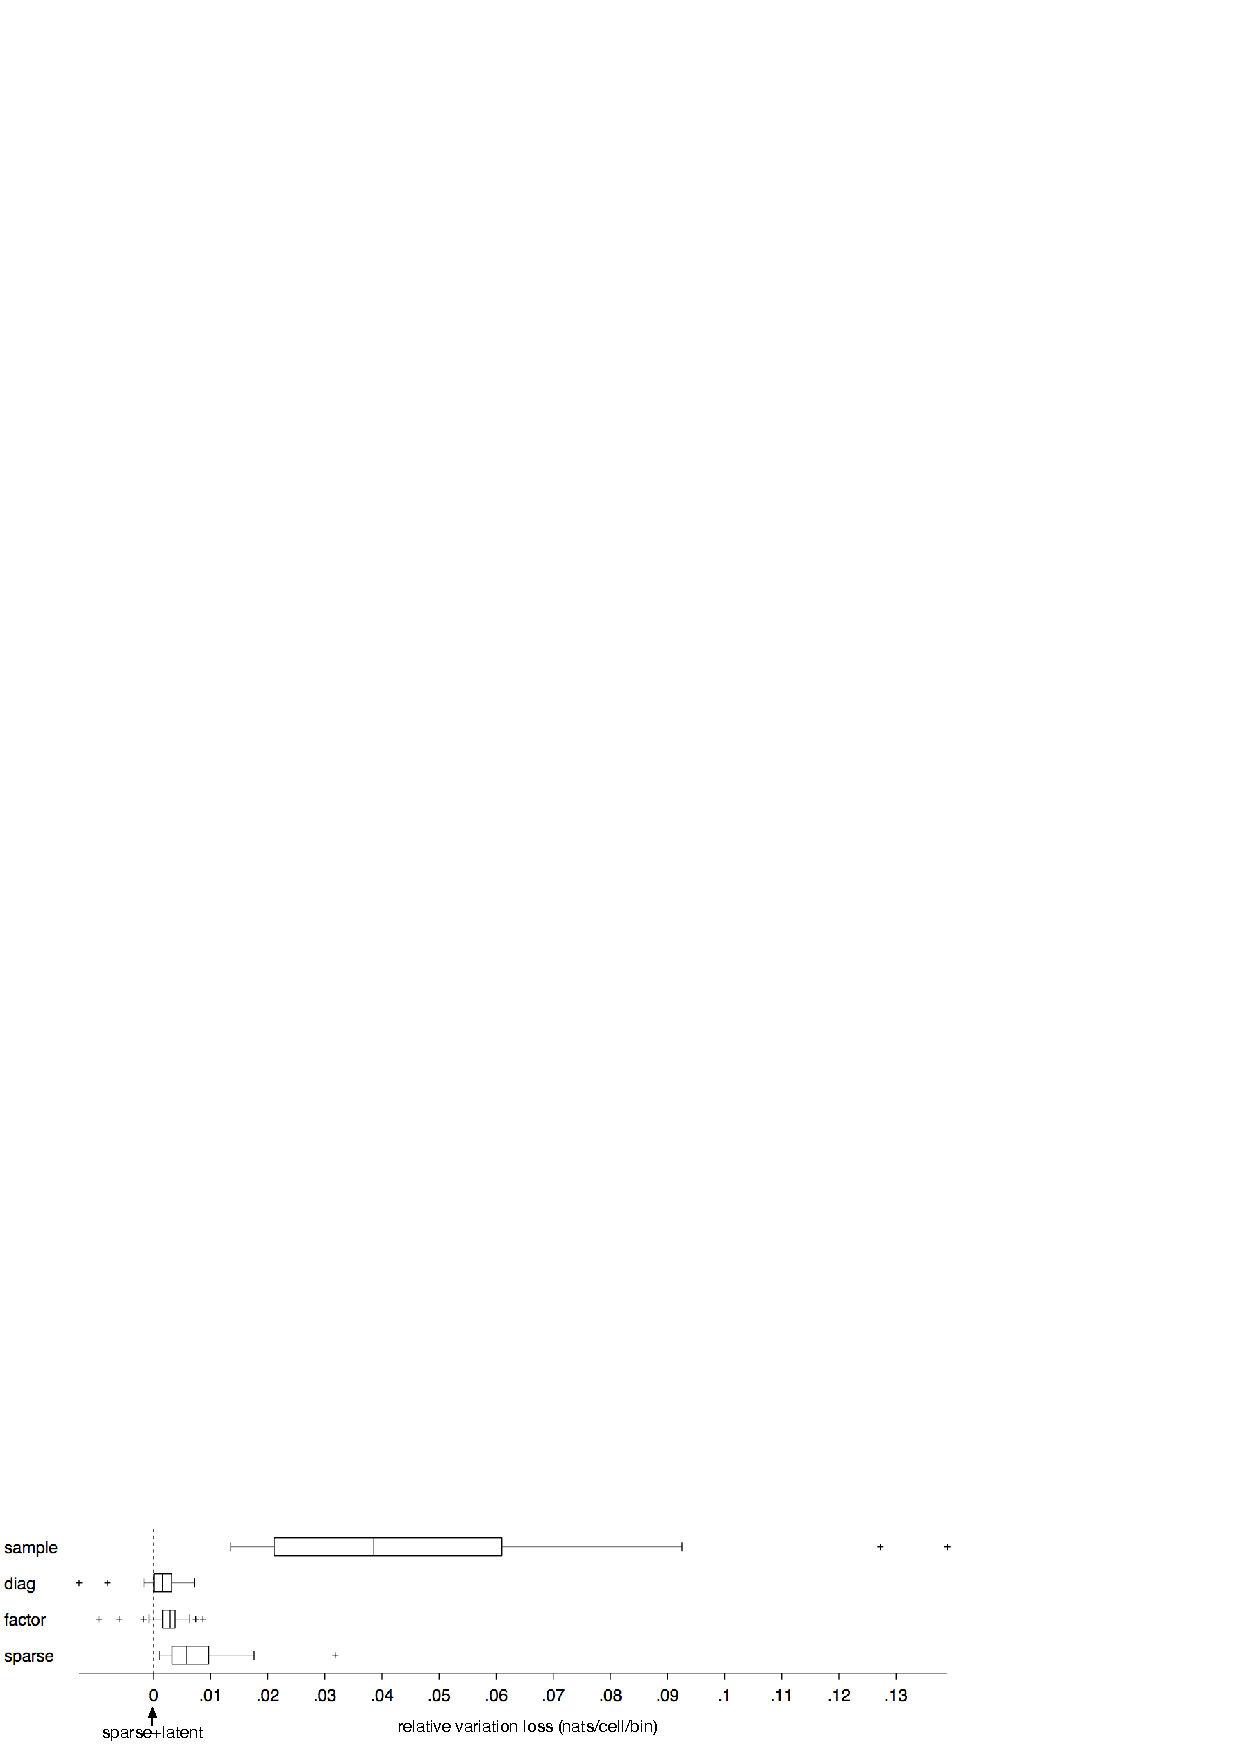
\includegraphics[width=0.5\textwidth]{figures/Figure4.pdf}
\caption{{\bf Estimator $\mathcal D$ (sparse+full-rank inverse covariance) dominates in dense recordings from primary visual cortex.}
{\bf A:}  Histogram of improvements in validation loss by covariance estimator $\mathcal D$ relative to the samle covariance matrix from the 31 imaged sites used in the study.  The vertical red line denotes the median improvment. 
{\bf B:} Improvements relative to estimator $\mathcal A$ (shrinkage toward the diagonal).
{\bf C:} Improvements relative to estimator $\mathcal B$ (shrinkage toward the factor model).
{\bf D:} Improvements relative to estimator $\mathcal C$ (sparse inverse covariance).
}\label{fig:04}
\end{figure}
Figure \ref{fig:04} showthe full matrix of all comparisons of the estimators.  The plots represents the histograms of the differences of the empirical loss between the pair of estimators for all 31 recorded sites.  When the differences are positive, the first estimate in the title outperforms the second estimate.

Of particular interest is the first row, which shows that all regularized estimates  outperformed the sample covariance estimate.  Even more informative is the last column, which shows that estimate D (sparse+lowrank) significantly outperformed all other estimates.

\subsection*{Relationship between functional covariance structure and circuit architecture}
\begin{figure}[htp]
\centering
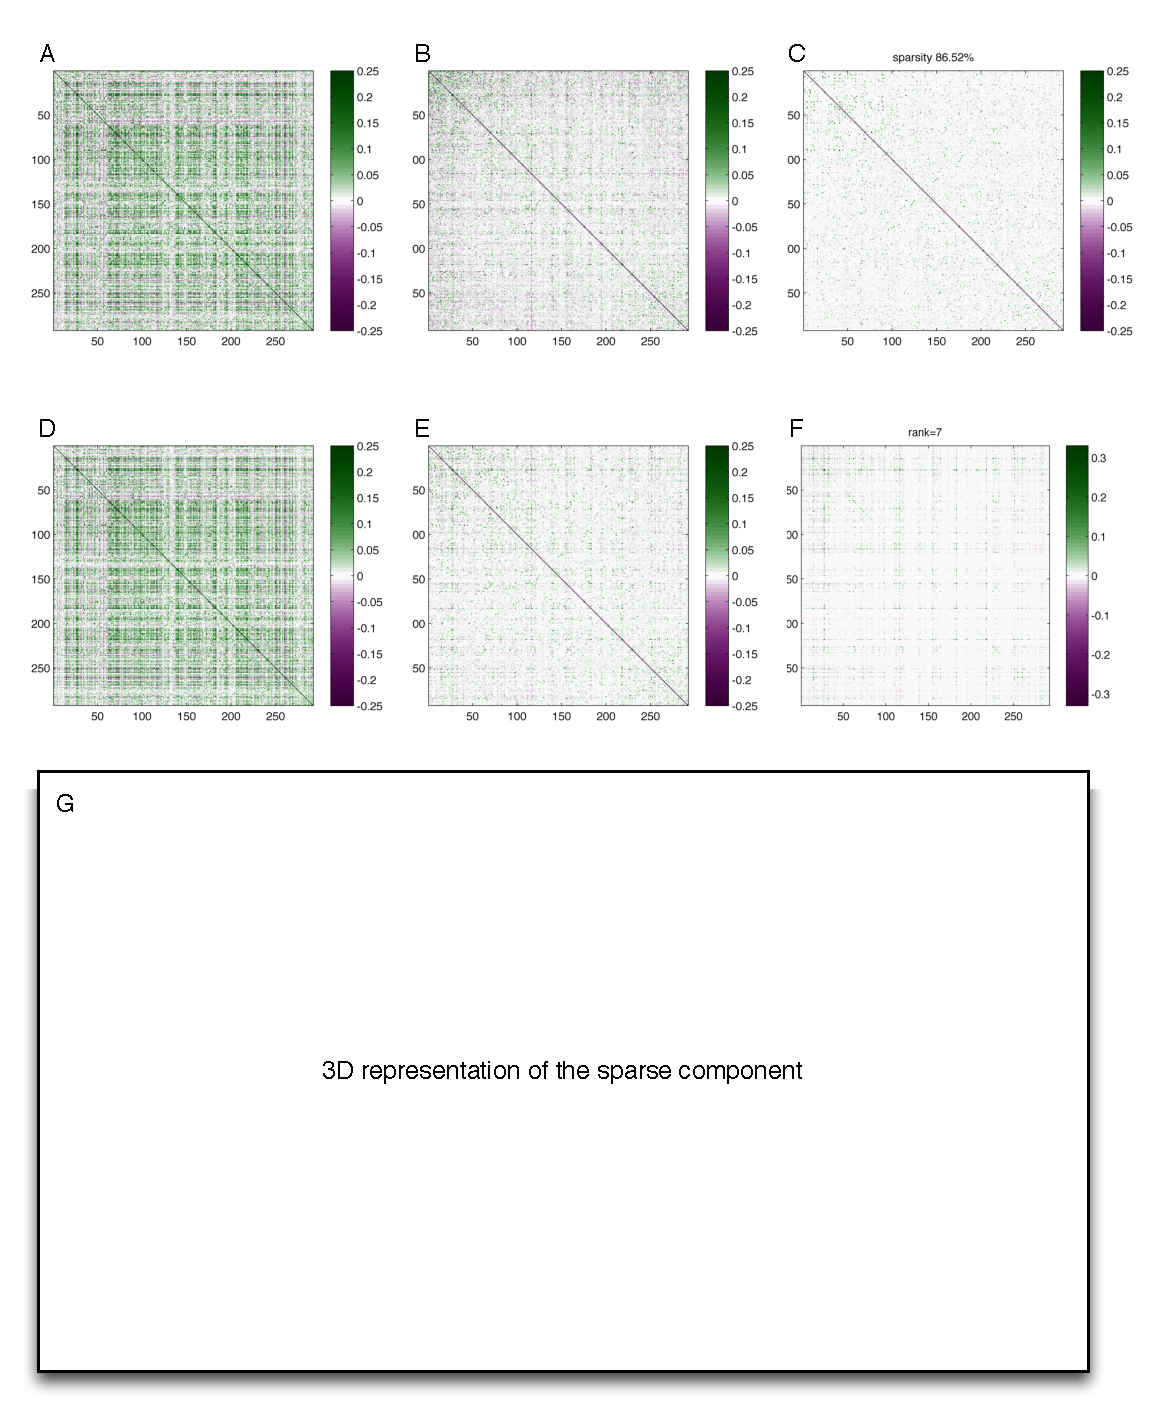
\includegraphics[width=1.0\textwidth]{figures/Figure5.pdf}
\caption{
Example of covariance structure revealed by the sparse+low-rank estimator and its relationship to the circuit arcitecture.
}
\label{fig:05}
\end{figure}

See Fig.~\ref{fig:05}.

\begin{figure}[htp]
\centering
\includegraphics{figures/Summary.pdf}
\caption{
Relationship between the structure of the estimate and the functional and spatial organization of the circuit.
{\bf A:} Average sample correlation, average partial sample correlation, and average partial correlation in the sparse+low-rank estimate for site in Fig.~\ref{fig:05} as a function of difference in cortical depth within the same column.
{\bf C:} Average sample correlation, average partial sample correlation, and average partial correlation in the sparse+low-rank estimate for site in Fig.~\ref{fig:05} as a function of lateral distance at the same cortical depth.
{\bf E,G:} Average sample correlation, and interaction probability obtained from the sparse+low-rank estimate as well as by thresholding the sample correlation matrix to equal sparsity as function of difference in cortical depnth and lateral distance.
{\bf I:} Average sample correlation, and interaction probability obtained from the sparse+low-rank estimate as well as by thresholding the sample correlation matrix to equal sparsity as a function of difference in preffered orientation.
}
\label{fig:06}
\end{figure}



\section*{Discussion}
\hl{The discussion section is not ready for any feedback. Currently it's just a trashbin with clips from scrapped versions of the introduction. -- Dimitri}

Fundamental questions in systems neuroscience concern the relationship between the function of neural microcircuits and their cytoarchitecture: circuit topology, cell types, and patterns of synaptic connectivity. 

Considerable progress has been made in sensory areas where the functional characterizations of cells are defined by their reproducible responses to external stimuli (reviewed in \citep{Reid:2012}). 

Many key questions in neuroscience revolve around the relationship between the cytoarchitecture of neural microcircuits and the functional organization of their activity \citep{Reid:2012}.  Investigators in this line of inquiry aim to construct networks of functional associations within groups of neurons inferred from observations of their activity under a variety of conditions.  The inferred functional network  could then related to the synaptic connectivity patterns, cell types, cell properties, or the cells' spatial arrangment in the attempt to uncover organizational principles of neural computation. In addition, the network itself can serve as subtrate for subsequent graph-theoretical analysis \citep{Feldt:2011}

Advances in electrophysiology and optical imaging have enabled simultaneous recordings from dozens to hundreds or thousands of cells. 
In particular, recent advances in two-photon imaging of calcium signals have allowed in vivo recordings from nearly every neuron brain-wide in zebrafish \citep{Leung:2013,Ahrens:2013} and in a 3D volume of a few hundred microns in diameter in mouse neocortex \citep{Katona:2012,Cotton:2013}.    
Ambitious projects currently under way aim to record the spiking activity of large fractions of cells from entire circuits and systems in behaving animals \citep{Alivisatos:2012}.  Direct observations of the population activity  of entire circuits open new possibilities for incisive statistical descriptions of the functional connectivity in the circuit.  


One general approach is to construct statistical models reflecting hypothesized models of neural circuit function, including temporal dynamics, nonlinear interactions between neurons, and background network activity \citep{Pillow:2008,Buonomano:2009,Yu:2009}. 
Another general approach is to search for alternative statistics that best describe the population activity without assuming a specific model.  Such evaluations rely on constructing surrogate datasets \citep{Okun:2012} or maximum-entropy distributions that reproduce the statistic of interest \citep{Ganmor:2011,Tkacik:2012} with subsequent testing of how well such constructs can reproduce other observed properties of population activity.

Such more sophisticated statistical descriptions are unlikely to entirely replace neural correlations as the initial descriptive statistic of population activity in experimental neuroscience. Neural correlations have several strengths that will ensure their continued prominence: (a) correlations are well established, familiar, and intuitive to most researchers in biological sciences, (b) correlations are easy to estimate as they are less susceptible to the curse of dimensionality than more sophisticated models, (c) correlations make relatively weak mechanistic assumptions (at the cost of not revealing many potentially important aspects), and (d) correlations serve as input into other models of population activity or decoding algorithms. 

Linear correlations between pairs of neurons are among the most common and familiar descriptions of functional associations in networks and of the collective activity of neuronal populations.  For example, it is tempting to consider the network constructed from the highest correlations in the recorded population (e.g.~\cite{Malmersjo:2013}) for subsequent graph-theoretical analysis \citep{Feldt:2011}.  In functional genomics, networks constructed from highest correlations are called \emph{relevance networks}.

However, pairwise correlations unreliable proxies of direct functional association such as direct synaptic connectivity as they can arise due to a wide variety of physiological interactions including direct synaptic interactions, indirect chains of synaptic connections, common inputs, correlations in inputs, synchrony, fluctuations in global network states, and others \citep{Shadlen:1998,Ostojic:2009,Pernice:2011,Schneidman:2006}.

Other experimental evidence suggests that detailed interactions in local microcircuits have only weak effects on overall population activity, which is then best characterized by collective features such as global population dynamics or population synchrony \citep{Okun:2012,Tkacik:2012,Tkacik:2013}.  From this point of view, the imporant aspects of the correlation structure lie it its global aspects, such as the eigenspectrum, while the individual pairwise correlations are not particularly meaningful.


% You may title this section "Methods" or "Models". 
% "Models" is not a valid title for PLoS ONE authors. However, PLoS ONE
% authors may use "Analysis" 
\section*{Materials and Methods}
\subsection*{Acquisition of calcium signals}
As described in \cite{Cotton:2013}



\subsection*{List of things to mention}

\begin{itemize}
\item How do we determine the mixing proportions $\lambda$ etc. Evaluation of likelihood/loss function on held-out validation set...

\item Define $L_1$ norm used for sparsification. Only off-diagonals are used?

\end{itemize}




% Do NOT remove this, even if you are not including acknowledgments
\section*{Acknowledgments}


%\section*{References}
% The bibtex filename
\bibliography{references.bib}


\section*{Figure Legends}
\TODO{presently embedded in the text}

%\section*{Tables}
%\begin{table}[!ht]
%\caption{
%\bf{Table title}}
%\begin{tabular}{|c|c|c|}
%table information
%\end{tabular}
%\begin{flushleft}Table caption
%\end{flushleft}
%\label{tab:label}
% \end{table}

\end{document}

